\documentclass[crop, tikz]{standalone}
\usepackage{tikz}
\usetikzlibrary{positioning}

\begin{document}
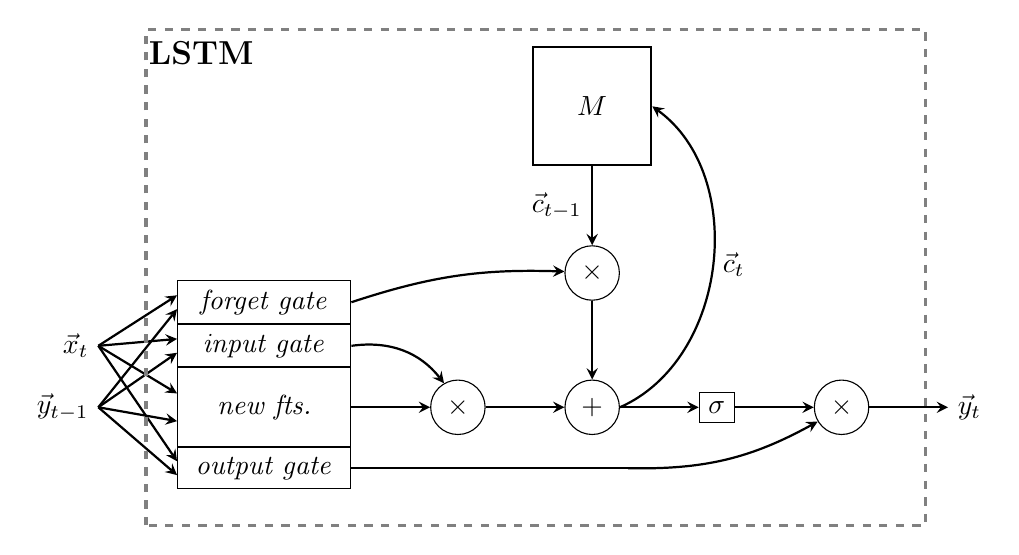
\begin{tikzpicture}
  \node[rectangle, draw, minimum width=2.2cm, minimum height=1cm] (FT) {\emph{new fts.}};
  \node[rectangle, above=0em of FT, draw, minimum width=2.2cm] (IG) {\emph{input gate}};
  \node[rectangle, above=0em of IG, draw, minimum width=2.2cm] (FG) {\emph{forget gate}};
  \node[rectangle, below=0em of FT, draw, minimum width=2.2cm] (OG) {\emph{output gate}};
  \node[left=of IG] (X) {$\vec{x}_t$};
  \node[left=of FT] (Y) {$\vec{y}_{t-1}$};

  \foreach \tgt/\dy in {FT/0.5em, IG/0.25em, FG/0.25em, OG/0.25em}
    \draw[-stealth, thick] (X.east) -- ([yshift=\dy]\tgt.west);
  \foreach \tgt/\dy in {FT/-0.5em, IG/-0.25em, FG/-0.25em, OG/-0.25em}
    \draw[-stealth, thick] (Y.east) -- ([yshift=\dy]\tgt.west);

  \node[circle, draw, right=of FT] (t1) {$\times$};
  \node[circle, draw, right=of t1] (pl) {$+$};
  \node[rectangle, draw, right=of pl] (th) {$\sigma$};
  \node[circle, draw, right=of th] (t2) {$\times$};
  \node[right=of t2] (Y1) {$\vec{y}_t$};
  \node[circle, draw, above=of pl] (t3) {$\times$};
  \node[rectangle, thick, draw, above=of t3, minimum width=1.5cm, minimum height=1.5cm] (M) {$M$};

  \foreach \from/\to in {FT/t1, t1/pl, pl/th, th/t2, t2/Y1, t3/pl}
    \draw[-stealth, thick] (\from) -- (\to);
  \draw[-stealth, thick] (M) -- node[left] {$\vec{c}_{t-1}$} (t3);
  \path[-stealth, thick] (IG.east) edge[bend left] (t1);
  \draw[thick] (OG.east) -- ([xshift=10em]OG.east);
  \path[-stealth, thick] ([xshift=10em]OG.east) edge[bend right=15] (t2);
  \path[-stealth, thick] (FG.east) edge[bend left=10] (t3);
  \path[-stealth, thick] (pl.east) edge[bend right=60] node[right] {$\vec{c}_t$} (M.east);

  \draw[very thick, dashed, gray] (-1.5, -1.5) rectangle (8.4, 4.8);
  \node at (-0.8, 4.5) {\large \bf LSTM};
\end{tikzpicture}
\end{document}
